\documentclass[11pt]{amsart}
\usepackage[marginratio=1:1, headheight=27pt,
footskip = 13pt, a4paper, total={6.5in, 9in}]{geometry}                % See geometry.pdf to learn the layout options. There are lots.
\geometry{letterpaper}                   % ... or a4paper or a5paper or ...
%\geometry{landscape}                % Activate for for rotated page geometry
%\usepackage[parfill]{parskip}    % Activate to begin paragraphs with an empty line rather than an indent
\usepackage{graphicx}
\usepackage[font=small,labelfont=bf]{caption} % Required for specifying captions to tables
%\usepackage{dirtytalk}
%\usepackage[version=3]{mhchem}
%\usepackage{subcaption}
%\usepackage{subfig}
%\usepackage{epstopdf}
\usepackage{booktabs}
\usepackage{caption}
\usepackage{subcaption}
\captionsetup{compatibility=false}
\usepackage[compact,small]{titlesec}
\usepackage{complexity}
%\usepackage[sc, osf]{mathpazo} % add possibly `sc` and `osf` options
%\usepackage{eulervm}
%\usepackage{textcomp}

\clubpenalty = 10000
\widowpenalty = 10000
%\usepackage[altbullet]{lucidabr}
\usepackage{float}
\usepackage{siunitx}
\usepackage[justification=centering]{caption}
\usepackage[
colorlinks = true,
urlcolor = blue
]{hyperref}
\usepackage{mathrsfs}
\usepackage{amssymb}
\usepackage{mathtools}
\usepackage{amsmath}
\usepackage{amsthm}
\renewcommand\qedsymbol{$\blacksquare$}

\usepackage[section]{placeins}
\DeclareGraphicsRule{.tif}{png}{.png}{`convert #1 `dirname #1`/`basename #1 .tif`.png}

%\usepackage[swedish]{babel}
\usepackage[T1]{fontenc}
\usepackage[utf8]{inputenc}

\usepackage{comment}
\usepackage{enumitem}
\titleformat{\section}[block]{\Large\scshape\centering}{\thesection.}{1em}{}
\titleformat{\subsection}[block]{\Large}{\thesubsection.}{1em}{}

\usepackage{pgfplots}
\pgfplotsset{compat = 1.15}

\usepackage[T1]{fontenc}

\usepackage{listings}
\lstset{basicstyle=\ttfamily,breaklines=true}
\usepackage{color} %red, green, blue, yellow, cyan, magenta, black, white
\definecolor{mygreen}{RGB}{28,172,0} % color values Red, Green, Blue
\definecolor{mylilas}{RGB}{170,55,241}

%\usepackage{times}
%\usepackage{kpfonts}
%\usepackage{txfonts}
%\usepackage{newtx}
%\usepackage{stix}
%\usepackage[osf,proportional]{libertine}
%\usepackage{lmodern}
%\usepackage[charter]{mathdesign}
\usepackage{libertine}
\usepackage{libertinust1math}
\usepackage[T1]{fontenc}
\usepackage{inconsolata}

\usepackage{microtype}
%\usepackage{stix}
\usepackage[compact,small]{titlesec}
\titleformat*{\section}{\large\scshape}

\titleformat*{\subsection}{\scshape}
\titleformat*{\subsubsection}{\large\bfseries\scshape}
%\renewcommand{\section}{\section*}
\newcommand{\ibits}{\{0, 1\}^*}
%\renewcommand{\familydefault}{\sfdefault}
\usepackage{marginnote}
\renewcommand*{\marginfont}{\color{red}\sffamily\footnotesize}
\usepackage{hyperref, xcolor}

%\usepackage{makeidx}
\definecolor{winered}{rgb}{0.5,0,0}
\hypersetup{
     pdfauthor={JAG},
     pdfsubject={Hyperlinks in LaTeX},
     pdftitle={main.tex},
     pdfkeywords={LaTeX, PDF, hyperlinks}
%    colorlinks=false,
     pdfborder={0 0 0},
%You can set individual colors for links as below:
colorlinks=true,
  linkcolor=winered,
urlcolor={winered},
filecolor={winered},
citecolor={winered},
allcolors={winered}
}

\usepackage[english]{babel}
\usepackage[
backend=biber,
style=numeric,
hyperref=true,
%natbib
]{biblatex}
\DeclareLanguageMapping{swedish}{swedish-apa}
\addbibresource{matkomkallorny.bib}

\usepackage{csquotes}
\usepackage[T1]{fontenc}
\usepackage{thmtools}
\usepackage{fancyhdr}
\usepackage{xcolor}

\usepackage{mdframed}
\newcommand{\ddx}{\frac{\text{d}}{\text{d}x}}
%\pagestyle{plain}
\newsavebox{\myheadbox}
\fancypagestyle{normalpage}
{
%\begin{flushright}
\lhead{
Jonas Conneryd
}
%\end{flushright}
\rhead{\url{conneryd@kth.se}}
\chead{MM7042 Mathematical Communication}
\cfoot{\thepage}
}
\fancyhf{}
\fancypagestyle{firstpage}
{
%\begin{flushright}
\lhead{
Jonas Conneryd \\ \url{conneryd@kth.se}}
%\end{flushright}
\rhead{970731-7559  \\
\the\year
}
\chead{\Large{\scshape{{Non-Constructive Algorithms} \\ \vspace{-4pt}\normalsize{MM7042 Mathematical Communication}}}}
\cfoot{\thepage}
}

\pagestyle{normalpage}

\definecolor{mybg}{rgb}{0.9,0.9,0.9}

\newmdtheoremenv[
backgroundcolor=mybg, %
innertopmargin =0pt , %
splittopskip = \topskip, %
skipbelow= 3pt, %
skipabove=3pt, %
topline=false,bottomline=false,leftline=false,rightline=false
%headfont=\scshape,
%bodyfont=\normalfont\itshape,
%shaded={bgcolor=\color{rgb}{0.9,0.9,0.9}}
]{theorem}{Theorem}

\newmdtheoremenv[
backgroundcolor=mybg, %
innertopmargin =0pt , %
splittopskip = \topskip, %
skipbelow= 3pt, %
skipabove=3pt, %
topline=false,bottomline=false,leftline=false,rightline=false
%headfont=\scshape,
%bodyfont=\normalfont\itshape,
%shaded={bgcolor=\color{rgb}{0.9,0.9,0.9}}
]{definition}{Definition}

\newmdtheoremenv[
backgroundcolor=mybg, %
innertopmargin =0pt , %
splittopskip = \topskip, %
skipbelow= 3pt, %
skipabove=3pt, %
topline=false,bottomline=false,leftline=false,rightline=false
%headfont=\scshape,
%bodyfont=\normalfont\itshape,
%shaded={bgcolor=\color{rgb}{0.9,0.9,0.9}}
]{remark}{Remark}


%\declaretheoremstyle[
%headfont=\scshape]{normalheaddef},
%shaded={bgcolor=\color{rgb}{0.9,0.9,0.9}}
\interfootnotelinepenalty=10000
%\title{\vspace{-2cm}\textbf{\textsf{ Homework 3}}}
\title{Non-Constructive Algorithms}
\author{
Jonas Conneryd \\
\url{conneryd@kth.se} \\
MM7042 Mathematical Communication\\
\the\year
}
\date{}
%\author{Jonas Conneryd \\
%conneryd@kth.se \\ 970731-7559}
\begin{document}
%\maketitle
\maketitle

\thispagestyle{plain}
%\theoremstyle{normalhead}
%\newtheorem{theorem}{Theorem}
%\theoremstyle{normalheaddef}
%\newtheorem{definition}{Definition}

\begin{abstract}
  The attitudes of mathematicians toward non-constructive results throughout the 20th and 21st centuries are exemplified and explored. L.E.J. Brouwer's school of intuitionism and its relation to the controversy regarding the first proof of the Hilbert Basis Theorem are briefly surveyed. The algorithmic implications of the Robertson-Seymour Theorem in Graph Theory are informally presented, and in particular that it implies a non-constructive result about algorithms, i.e. a proof that an effective algorithm exists for a certain class of computational problems that does not provide the algorithm itself. The discussions surrounding this fact are contrasted to those surrounding those regarding the Hilbert Basis Theorem.
\end{abstract}



\section{Introduction}
In modern mathematics, the notion of what constitutes a mathematical proof seems to be clear enough that results can be published in journals, prizes can be awarded, and incorrect proofs can be refuted. (However, it seems that when you ask mathematicians what exactly\cite{seymourGraphMinorsXIII1995} \cite{vanattenLuitzenEgbertusJan2020} a proof is, you're likely to get an answer similar to what Louis Armstrong is supposed to have replied when asked to define jazz: ''If you have to ask, you'll never know''). But this wasn't always as universally agreed upon; in the start of the 20:th century, powerful but non-constructive results sparked a debate among mathematicians about which proof methods are valid. While this debate was eventually essentially settled in favor of non-constructive results, constructive mathematics seems to have gotten a spiritual successor in the form of algorithms research. Surely, to prove a result of the form ''There exists an algorithm that solves a certain computational problem with a certain efficiency'', what else could one do than provide an algorithm that solves the problem at hand, and prove that it does so with the claimed efficiency? This essay will survey a result which goes about proving such a result in a non-constructive way.

\section{The Result that Started it All}
Up until the end of the 19:th century, essentially all mathematical existence proofs had been constructive in nature. Although Cantor seems to have produced some non-constructive existence results, it was the proof of Hilbert's Basis Theorem in 1888 that initially sparked a debate about the nature of proof. Hilbert's Basis Theorem states that
\begin{theorem}
If $R$ is a Noetherian ring, then $R[X]$ is a Noetherian ring.
\end{theorem}
To some readers, this result is second nature; to others it says nothing at all. What matters here is however \emph{how} he proved it. To prove this result, one needs to show that a finite collection of mathematical objects with a set of certain specifications exists. Hilbert did so without actually \emph{constructing} them, which was novel at the time. The result itself is very powerful and the basis of many further results in algebra.

\section{The Objections}
A cohort of mathematicians that were sympathetic towards the constructivist view of mathematics, in which a proof of existence is one where the object of interest is actually constructed, were not convinced by this proof. Paul Gordan, known to all students of quantum mechanics for ''Clebsch-Gordan coefficients'', is supposed to have said about this result, albeit with unclear intention, that

''This is not mathematics; this is theology!''.

Poincaré also put forward sharp criticism, but perhaps the fiercest opponent was L. E. J. Brouwer (of Brouwer's fixed point theorem fame) and the followers of his \emph{intuitionist} view of mathematics. There are other schools of constructive mathematics (for an overview, see Section 3 in \cite{bridgesConstructiveMathematics2018}) but in consideration of space, only intuitionism is (briefly) surveyed in this essay.

\section{What is intuitionism?}
Hilbert was a proponent of \emph{formalism} \cite{zachHilbertProgram2019}, which maintained the view that mathematics is essentially a game about symbol manipulation in which the rules are clear and well defined, and results obtained through these rules are, in some sense, objectively true within the bounds of the game\footnote{This is obviously, and in this medium probably unavoidably, a gross simplification of the ideas Hilbert subscribed to in the philosophy of mathematics. For a more detailed account and its connection to the project to axiomatize mathematics initiated by Hilbert, see \cite{zachHilbertProgram2019}.}. Brouwer, on the other hand, thought that mathematics is inherently a subjective activity - the result of constructive mental activity by humans \cite{iemhoffIntuitionismPhilosophyMathematics2020}. This implies in particular that mathematical truth is subjective, with the following consequence: A mathematical object is considered a product of a construction produced by a mind, and therefore existence of an object is \emph{equivalent} to its possibility of being constructed. This stands in sharp contrast to the usual approach, in which it is valid to prove existence of an object through refuting its non-existence. Put succinctly, yet possibly a bit crudely, intuitionists in the sense of Brouwer refute the validity of the \emph{law of excluded middle}: That for any proposition, either that proposition or its negation are true \cite{iemhoffIntuitionismPhilosophyMathematics2020}.

\section{Algorithmic research and non-constructivism}
The mathematics of the 21st century seems to not be especially concerned with issues similar to those discussed in the Hilbert-Brouwer controverst. Indeed, the debate over the law of excluded middle seems to have been decisively settled in favor of it, as most any practicioner of mathematics would be ready to confirm. But it seems that mathematics whose chief concern is actual construction of mathematical objects has made somewhat of a comeback with the advent of the mathematical theory of computation, more precisely the mathematical study of algorithms.

Complexity Theory, that part of mathematics that deals with classifying computational problems after how efficiently they can be solved by algorithms. In Complexity Theory, the notion of an ''effective'' algorithm is defined to be an algorithm whose running time scales polynomially with the size of the input to the algorithm\footnote{For a discussion on this definition of ''effectiveness'' in Complexity Theory, see Section 1.5 in  \cite{aroraComputationalComplexityModern2009a}. }. Complexity Theory is a proper subfield of mathematics, and results in Complexity Theory are in general answers to questions of the form
\begin{center}
\emph{Does there exist an algorithm that solves $\langle$\emph{computational problem}$\rangle$ in $\langle$\emph{conjectured efficiency}$\rangle$?}
\end{center}
How would one prove an affirmative result in Complexity Theory? The answer seems to invariably be to construct an algorithm that indeed solves the computational problem at hand with sufficient efficiency\footnote{Negative results are another story. A general way to prove negative results in Complexity Theory is worth at least a million dollars in prize money, cf. \cite{VsNPProblem}.}. Nonetheless, it turns out that there are non-constructive existence results in Complexity Theory, and the remainder of this essay aims to introduce one such result (or rather, an infinite collection of such results).

\section{The Robertson-Seymour theorem}
The results in question are the algorithmic implications of the \emph{Robertson-Seymour Theorem}, which follow from the combination of this theorem with another theorem, also by Robertson and Seymour. Both results are introduced in this essay. The results concern \emph{graphs}, which are collections of \emph{vertices} with \emph{edges} drawn between them. Some definitions are needed to state both theorems by Robertson and Seymour. It should be noted that the definitions and theorem statements in this essay are mostly of the more informal kind, since a more rigorous treatment of the subject would demand a great deal more space to convey essentially the same content.

\begin{definition}[Informal]
A \emph{graph} $G = (V,E)$ is a collection of vertices (points) and edges (lines between the points).
\end{definition}
Graphs model pairwise relations between objects and are of immense importance in algorithms research and mathematical modelling, as well as very fascinating mathematical objects in their own right\footnote{A rigorous introduction to the subject covering most of its major developments, including a more detailed exposition of the results covered in this essay, is \cite{diestelGraphTheory2017}.}. Two very simple examples of graphs can be found in Figure \ref{fig:graphs1}.
\begin{figure}[h!]
  \begin{center}
    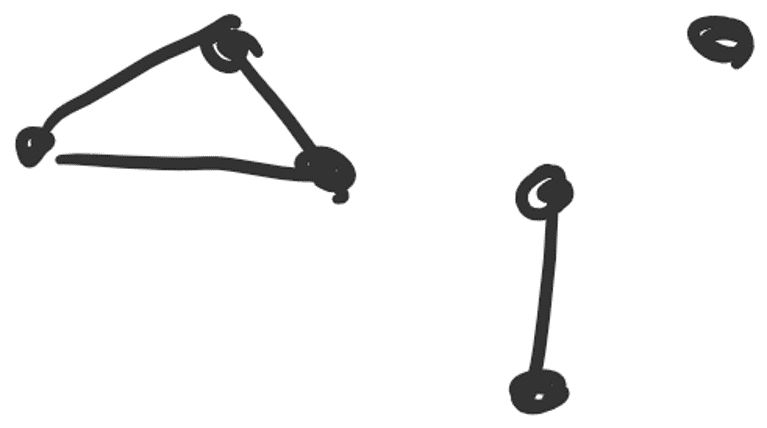
\includegraphics[width = 0.25\textwidth]{graf2.png}
  \end{center}
    \caption{Two graphs with three vertices. The graph to the left has three edges and the the graph to the right has two edges.}

  \label{fig:graphs1}
\end{figure}


It should be noted that the visual representation of the graph is immaterial; the two graphs in Figure \ref{fig:graphs2} are the same graph.
\begin{figure}[h!]
  \begin{center}
    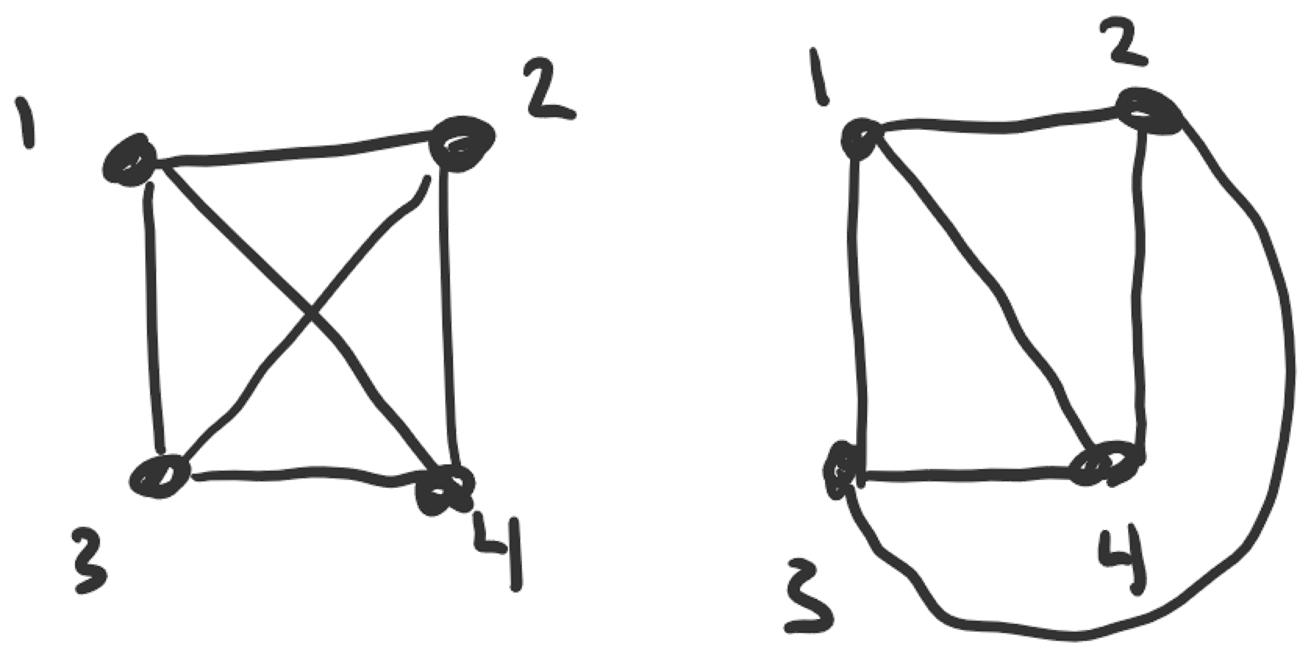
\includegraphics[width = 0.25\textwidth]{graf.png}
  \end{center}
    \caption{Two equivalent visual representations of the unique graph with four vertices and four edges.}

  \label{fig:graphs2}
\end{figure}

The goal of Graph Theory is, naturally, to study properties defined on graphs and to study how different graphs relate to each other. One example of a graph property is whether it is possible to draw the graph on the plane without any of its edges intersection, in which case we say the graph is \emph{planar}. An example of a graph relation, which is the relation of interest in this essay, is when a graph $H$ is a \emph{minor} of another graph $G$.

\begin{definition}
Let $H$ and $G$ be graphs. If we can form $H$ from $G$ by deleting vertices, deleting edges and contracting two edge-connected vertices into one, we say that $H$ is a \emph{minor} of $G$. The process of deleting vertices, deleting edges and contracting two edge-connected vertices into one is denoted by \emph{taking minors}.
\end{definition}
A visual representation of each of the operations allowed under taking minors can be seen in Figure \ref{fig:minoroperations}.
\begin{figure}[h!]
  \centering
      \begin{subfigure}[t]{0.3\textwidth}
          \centering
          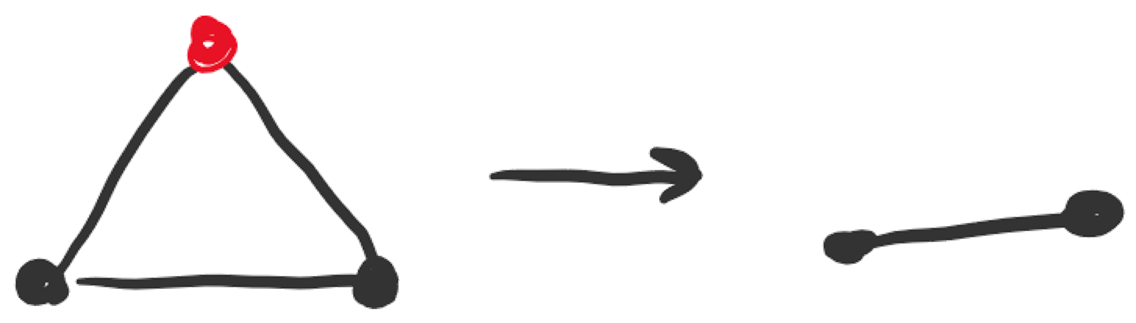
\includegraphics[width = \textwidth]{deletevertex.png}
          \caption{Deleting a vertex.}
      \end{subfigure}%
       \hfill
      \begin{subfigure}[t]{0.3\textwidth}
          \centering
          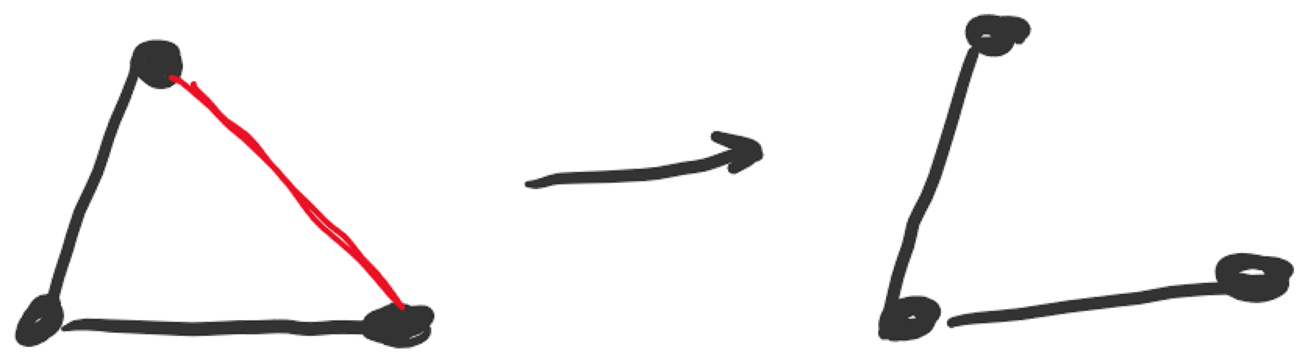
\includegraphics[width = \textwidth]{deleteedge.png}
          \caption{Deleting an edge.}
      \end{subfigure}
       \hfill
      \begin{subfigure}[t]{0.3\textwidth}
          \centering
          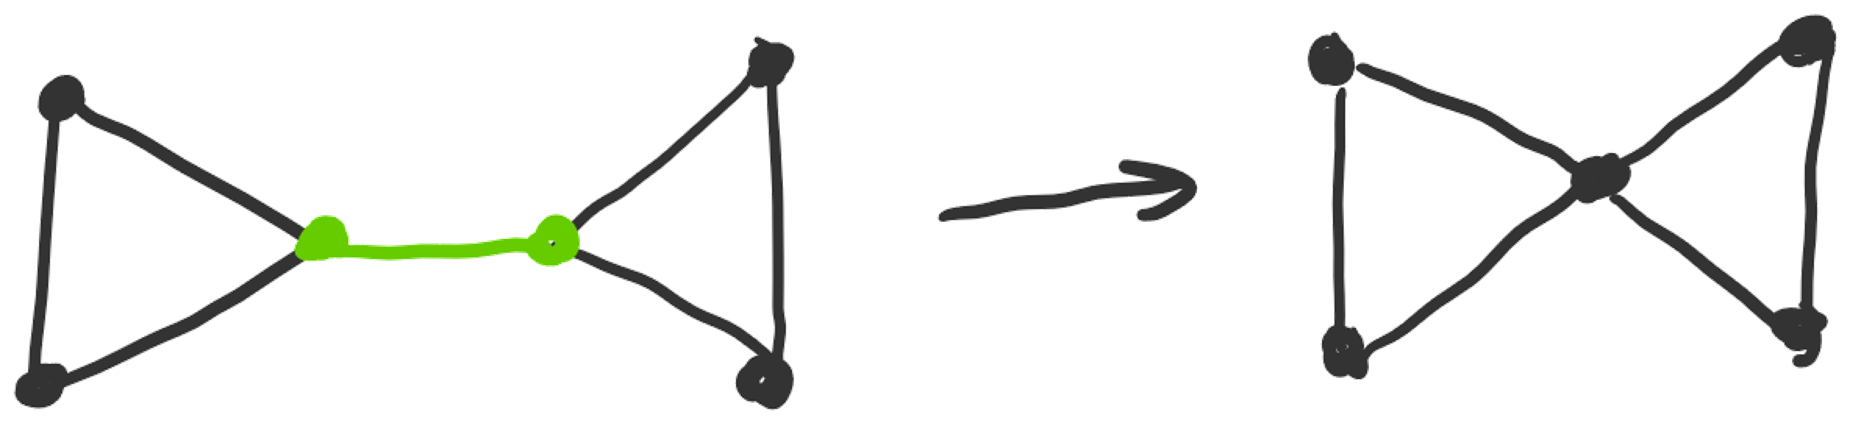
\includegraphics[width = \textwidth]{contractedge.png}
          \caption{Contracting an edge.}
      \end{subfigure}
      \caption{Operations allowed when taking minors.}
      \label{fig:minoroperations}
\end{figure}

 Planarity is one of many properties a graph can possess that are retained under taking minors. Such graph properties are called \emph{minor-closed}. The Robertson-Seymour Theorem relates to such properties of graphs, and the concepts defined so far are suficcient to state it.

\begin{theorem}[Robertson-Seymour]
Suppose a graph property $\mathcal{P}$ is retained when taking minors. Then there is a finite list of graphs such that a graph $G$ has property $\mathcal{P}$ if and only if none of the graphs in the list can be formed from $G$ by taking minors\footnote{For a detailed account of this theorem (albeit not its full proof, for good reason), see Chapter 12 of \cite{diestelGraphTheory2017}.}.
\end{theorem}

\begin{remark}
  The graphs in the finite list described in the Robertson-Seymour Theorem belonging to a graph property $\mathcal{P}$ are called the \emph{forbidden minors} of $\mathcal{P}$.
\end{remark}

At first glance, the (extremely deep) ramifications of the Robertson-Seymour Theorem might not be apparent. It should also be noted that despite the seemingly simple statement of the theorem, its proof took 20 years and comparably many long journal articles totalling over 500 pages, to complete \cite{RobertsonSeymourTheorem2020}. Its power in the field of Complexity Theory will become apparent when combined with the following result by the same authors.
\begin{theorem}
Let $H$ be a fixed graph, and let $G= (V, E)$ be an arbitrary graph. Then there is an algorithm that decides if $H$ is a minor of $G$ whose running time scales polynomially with the number of vertices of $G$.
\end{theorem}
For a proof of this theorem, see \cite{seymourGraphMinorsXIII1995}. The proof is constructive in that it is a description of an algorithm that checks whether $H$ is a minor of $G$ in the alotted time. The analysis of the running time of the algorithm takes around 50 pages.


Together, Theorem 2 and Theorem 3 will yield a very strong result about algorithms regarding the computational problem of determining whether a graph $G$ has some property $\mathcal{P}$ which is minor-closed. We know by Theorem 2 that belonging to $\mathcal{P}$ is some finite list of graphs such that a graph $G$ has property $\mathcal{P}$ if and only if none of the graphs in the list is a minor of $G$. This list is the same regardless of the input graph, so we have to check a constant, finite number of cases to determine whether $G$ has property $\mathcal{P}$. By Theorem 3 we know that we can check each case in time polynomially related to the number of vertices of $G$, so the total number of cases can in fact also be checked in time polynomially related to the number of vertices of $G$, since a constant times a polynomial is still a polynomial. Therefore, we have the following algorithmic result:
\begin{theorem}
Determining whether a given graph $G=(V, E)$ has a property $\mathcal{P}$ that is closed under taking minors can be done in time polynomially related to the number of verices of $G$.
\end{theorem}

We already saw one example of a minor-closed property, namely planarity. More generally, one (out of many) family of minor-closed properties of a graph is being able to be drawn on a surface, such as a sphere or donut surface, without edges crossing \cite{GraphMinor2020}.

This is indeed a non-constructive existence proof of an efficient 

\section{Non-constructive existealgorithms}
So we have a theorem that says that to determine whether a graph has a certain property, a finite amount of cases have to be checked, and each case can be checked efficiently. But the Robertson-Seymour theorem says nothing about which these cases are; for all but the most elementary cases, we have no idea which graphs are in the list of ''forbidden minors''. As an example, the property that a graph can be drawn on a donut surface without lines intersecting turns out to be retained while taking minors, but the list of forbidden minors has been proved to be of size at least 17000, and there is no guarantee that this list is exhaustive. To add insult to injury, the algorithm that decides whether a graph $G$ has another fixed graph $H$ as a minor turns out to be so terribly slow in practise that running it

\section{The debate around this result}
While no new schools of Complexity Theory were started after this result appeared (to my knowledge), this result called into question whether the categorizations we have chosen for when to call an algorithm ''efficient'', and really, how we prove things in Complexity Theory, are really the right ones. For one, the case for constructive results is much stronger when it comes to algorithms; If the purpose of Complexity Theory is to find efficient algorithms for important problems, what good is it, really, to know that an algorithm exists if we have no way of constructing, let alone use it? Also, can an algorithm really be called ''efficient'' if running it will take many times the lifetime of the universe for the most trivial of cases? Indeed, one famous computer scientist is supposed to have said about this result: ''This is not computer science. This is a mathematical curiosity!''. This result has its own version of Govan's saying.

\section{Concluding remarks}
In my opinion, Complexity Theory took a significant step away from computer science and toward mathematics with this result (which came from pure mathematics, interestingly enough!). While it is wonderfully useless in itself, it makes one reconsider preconceived notions and intuition related to what an algorithm is. As a fan of all things useless and interesting, I hope for more, not fewer, results of this kind in the future.

\newpage
\printbibliography
\end{document}
